\documentclass[a4paper,11pt]{article}

\usepackage[english]{babel}
\usepackage[utf8x]{inputenc}
\usepackage{amsmath}
\usepackage{graphicx}
\usepackage{cite}
\usepackage{hyperref}
\usepackage{fullpage}
% \usepackage{apacite}
\setlength{\parskip}{1.2ex}
\begin{document}

\title{Open Information System: Conceptual schema}
\author{Thomas Perale -- 0546990\\Maximilien Romain -- 0543411\\Felipe Rojas -- 0542569\\Lehal Sherik -- 0543118}
\date{27 October 2017}

\maketitle

\section{Project subject}

\begin{itemize}
  \item Ebook shop
  \item Various ebook types
  \item Searchable
  \begin{itemize}
    \item Authors
    \item ISBN
    \item Edition
    \item Title
    \item Category
    \item Year
  \end{itemize}
  \item Pricing
\end{itemize}

\section{Database usecases}

\begin{itemize}
  \item The user register by choosing a “username” and a “password” and “email” if the username is not already taken in the database we create a new entry with the password and username or it’s taken we ask to choose another username.
  \item The user login the website using username and password we check in the “User” table if the username exist if it exist we check if the password match.
  \item When the user search for a book by default it try to match the user query with the title and the author name in the database.
  \item The user can search for a book using more in deep parameter like the title, category, authors, price, isbn, etc… It try to match those parameters with the corresponding field in the “Book” table.
  \item If an user find a book interesting they can buy it when it’s done the bought items are stored “Purchases” table.
  \item User can filters books by categories, the database only retrieve the matching category when we filter categories.
  \item Books are added on the database only by the admin it’s mandatory to fulfill every field to create a new book on the database.
\end{itemize}

\section{ER Schema}

\begin{center}
  \makebox[\textwidth]{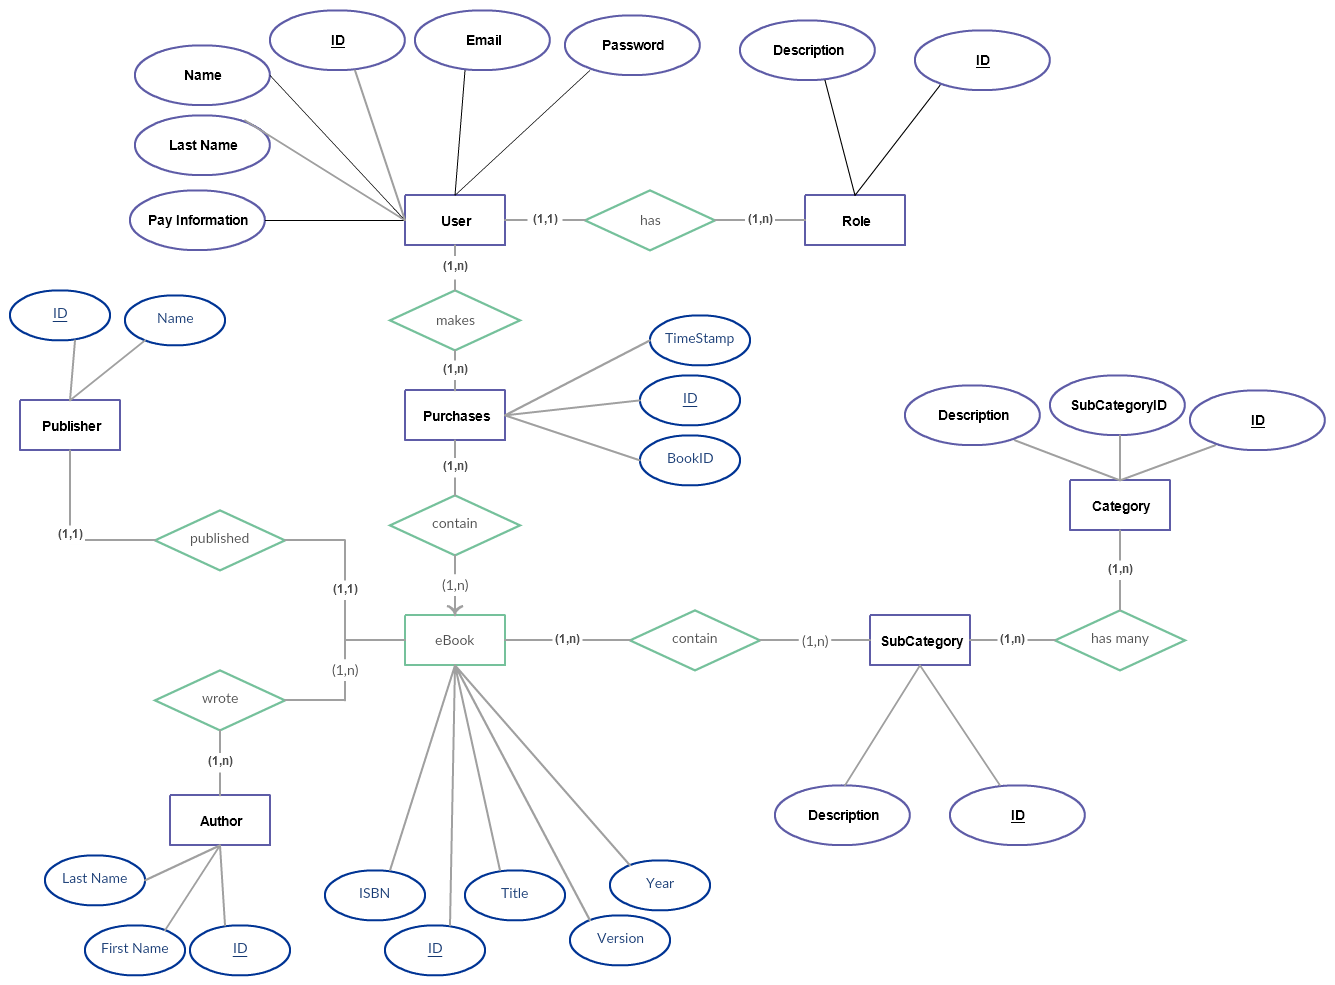
\includegraphics[width=\paperwidth]{er.png}}
\end{center}

\end{document}
